{\tiny \documentclass[
%parspace, % Add vertical space between paragraphs
%noindent, % No indentation of first lines in each paragraph
%nohyp,	   % No hyphenation of words
%twoside,  % Double sided format
%draft,    % Quicker draft compilation without rendering images
%final,    % Set final to hide todos
]{elteikthesis}[2024/04/26]


% The minted package is also supported for source highlighting
% See elteikthesis_minted.tex for example
%\usepackage[newfloat]{minted}
\usepackage{enumitem}
\usepackage{tikz}
\usetikzlibrary{arrows}

% Document's metadata
\title{Mérték, integrál, valószínűség} % title
\subtitle{\circled{7} Vizsgatétel}

% The document
\begin{document}
	
	% Set document language
	\documentlang{hungarian}
	
	\section{Stieltjes-féle kvázimérték}
	
	A továbbiakban legyen \( \func{\varphi}{\R}{\R} \) egy monoton növekedő függvény, 
	\marginnote{
		Tehát az itt szereplő halmazfüggvény
		\[
			\func{m}{\mathbf{I}}{[0, +\infty)}
		\]
	}
	valamint
	\[
	%	\func{m}{\mathbf{I}}{[0, +\infty)}, \quad
		m(\emptyset) \coloneq 0, \quad
		m \bigl( [x, y) \bigr) \coloneq \varphi(y) - \varphi(x)
		\qquad (x, y \in \R, \ x < y).
	\]
	Az itt szereplő \( \mathbf{I} \) halmazrendszer az üres halmazt, 
	valamint az \( \R \) balról zárt, jobbról nyílt intervallumait tartalmazza, 
	\( \mathcal{I} \) pedig az \( \mathbf{I} \) félgyűrű által generált gyűrű, azaz
	\[
		\mathbf{I} \coloneq 
		\setc[\Big]{ \emptyset, [a, b) \subseteq \R }{ a, b \in \R, \ a < b }, \qquad
		\mathcal{I} \coloneq \mathcal{G}(\mathbf{I}).
	\]
	
	\begin{theorem}{}{}
		A most bevezetett \( \widetilde{\mu}_\varphi \) kvázimérték \( \iff \)
		\( \varphi \) balról folytonos.
	\end{theorem}
	\begin{proof}\,\\
		\Ifstep
		Indirekt tegyük fel,
		\marginnote{
			Ami most azzal ekvivalens, hogy
			\[
				\lim_{t \to x-0} \varphi(t) \neq \varphi(x).
			\]
		}
		hogy a \( \varphi \) nem folytonos balról egy \( x \in \R \) helyen.\\[6pt]
%		Mivel a \( \varphi \) elve monoton növekedő, ezért ez azt jelenti, hogy
%		\[
%			\lim_{t \to x-0} \varphi(t) < \varphi(x).
%		\]
		Legyen az \( \func{(x_n)}{\N}{\R} \) szigorúan monoton növekedő, \( \lim(x_n) = x \).
		Ekkor
		\[
			[x_0, x) = \bigcup_{n=0}^{\infty} [x_n, x_{n + 1})
		\]
		egy páronként diszjunkt felbontás, 
		ezért a \(  \widetilde{\mu}_\varphi \) szigma-additivitása miatt
		\marginnote{
			Itt kihasználjuk, hogy mivel léteznek a
			\[
				\lim_{t \to x-0} f(t), \quad
				\lim_{n \to \infty} x_n = x
			\]
			határértékek, ezért az átviteli-elv miatt
			\begin{equation}\label{eq:stieltjes-01}
				\lim_{n \to \infty} f(x_n) = 
				\lim_{t \to x-0} f(t).
				\tag{\( * \)}
			\end{equation}
		}
		\begin{align*}
			\widetilde{\mu}_\varphi \bigl( [x_0, x) \bigr)
			&= \sum_{n=0}^{\infty} \widetilde{\mu}_\varphi \bigl( [x_n, x_{n + 1}) \bigr)
			 = \sum_{n=0}^{\infty} \Bigl( \varphi( x_{n + 1} ) - \varphi( x_n ) \Bigr) \\
			%= \bigl( \varphi( x ) - \varphi( x_0 ) \bigr) \\
			&= \lim_{n \to \infty} \sum_{k=0}^{n - 1} 
			   \Bigl( \varphi( x_{k + 1} ) - \varphi( x_k ) \Bigr)
			 = \lim_{n \to \infty} 
			   \bigl( \varphi( x_n ) - \varphi( x_0 ) \bigr) \\[3pt]
			&\overset{\text{\ref{eq:stieltjes-01}}}{=}
			   \lim_{t \to x-0} 
			   \bigl( \varphi( t ) - \varphi( x_0 ) \bigr)
		\end{align*}
		Ugyanakkor az \( m \) halmazfüggvény definíciójából adódóan
		\marginnote{
			Vagyis az alábbi ellentmondást kapjuk:
			\[
				\lim_{t \to x-0} \varphi(t) = \varphi(x).
			\]
		}
		\[
			\widetilde{\mu}_\varphi \bigl( [x, x_0) \bigr) =
			\varphi( x ) - \varphi( x_0 ) =
			\lim_{t \to x-0}  \bigl( \varphi( t ) - \varphi( x_0 ) \bigr).
		\]
		Ez pedig pontosan azt jelenti, hogy a \( \varphi \) balról folytonos az \( x \)-ben.
		
		\vspace{6pt}
		\hrule
		\vspace{6pt}
		
		\newpage
		\Backifstep
		Azt kell megmutatni, hogy a \( \widetilde{\mu}_\varphi \) szigma-additív.
		Ehhez elég lenne azt belátni, hogy az \( m \) szigma-additív.
		Mivel az \( m \) előmérték, ezért tetszőleges
		\[
			a_n, b_n \in \R, \quad a_n < b_n \quad (n \in \N), \qquad 
		%	\bigcup_{n = 0}^{\infty} [a_n, b_n) = [a, b) \in \mathbf{I}
			\mathbf{I} \ni [a, b) = \bigcup_{n = 0}^{\infty} [a_n, b_n)
		\]
		páronként diszjunkt felbontás esetén
		\marginnote{Lásd előmértékek tulajdonságai.}
		\[
			\sum_{n=0}^{\infty} m \bigl( [a_n, b_n) \bigr) \leq
			m \Biggl( \, \bigcup_{n = 0}^{\infty} [a_n, b_n) \Biggr) =
			m \bigl( [a, b) \bigr).
		\]
		Most megmutatjuk, hogy fennáll a fordított irányú egyenlőtlenség is, azaz
		\[
			m \bigl( [a, b) \bigr) = 
			\varphi(b) - \varphi(a) \leq
			\sum_{n=0}^{\infty} \bigl( \varphi(b_n) - \varphi(a_n) \bigr).
		\]
		Válasszunk egy tetszőleges \( c \in (a,b) \) számot, lásd \ref{fig:stieltjes-01}. ábra.
		Mivel a \( \varphi \) balról folytonos és monoton nő,
		\marginnote{%
			\centering
			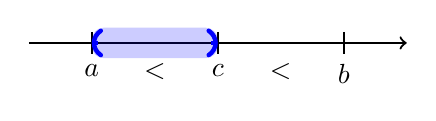
\begin{tikzpicture}[scale=8]
				\draw[->, thick] (-0.1,0) -- (0.5,0);
				
				\foreach \x in {0.1, 0.3}
					\draw (\x,-0.5pt) node[below] {$<$};
					
				\foreach \x/\xtext in {0/$a$,0.2/$c$,0.4/$b$}
					\draw[thick] (\x,0.5pt) -- (\x,-0.5pt) node[below] {\xtext};
					
				\draw[(-, ultra thick, blue] (0,0) -- (0.01,0);
				\draw[-), ultra thick, blue] (0.19,0) -- (0.2,0);
				\fill[opacity = 0.2, blue,rounded corners=1ex] (0,-.16ex) -- (0.2, -.16ex) -- (0.2, .16ex) -- (0,.16ex) -- cycle;
			\end{tikzpicture}
			\vspace{-\baselineskip}
			\captionof{figure}{}\label{fig:stieltjes-01}
		}[-\baselineskip]
		ezért bármely \( \varepsilon > 0 \)-hoz és \( n \in \N \) indexhez
		%
		\begin{equation}\label{eq:stieltjes-02}
			\exists \,\widetilde{a}_n < a_n \, \colon \ \quad
			\varphi( a_n ) - \varphi( \widetilde{a}_n ) < \frac{\varepsilon}{2^n}
			\tag{\( ** \)}
		\end{equation}
		%
		fennáll, lásd \ref{fig:stieltjes-02} ábra.
		\marginnote{%
			\centering
			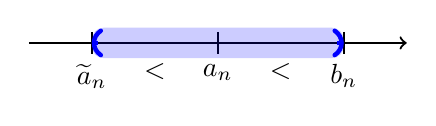
\begin{tikzpicture}[scale=8]
				\draw[->, thick] (-0.1,0) -- (0.5,0);
				
				\foreach \x in {0.1, 0.3}
				\draw (\x,-0.5pt) node[below] {$<$};
				
				\foreach \x/\xtext in {0/$\widetilde{a}_n$,0.2/$a_n$,0.4/$b_n$}
				\draw[thick] (\x,0.5pt) -- (\x,-0.5pt) node[below] {\xtext};
				
				\draw[(-, ultra thick, blue] (0,0) -- (0.01,0);
				\draw[-), ultra thick, blue] (0.39,0) -- (0.4,0);
				\fill[opacity = 0.2, blue,rounded corners=1ex] (0,-.16ex) -- (0.4, -.16ex) -- (0.4, .16ex) -- (0,.16ex) -- cycle;
			\end{tikzpicture}
			\vspace{-1\baselineskip}
			\captionof{figure}{}\label{fig:stieltjes-02}
		}[-\baselineskip]
		Ez alapján világos, hogy
		\[
		%	[a, c) \subset
			[a, c] \subseteq 
			\bigcup_{n=0}^{\infty} ( \,\widetilde{a}_n, b_n ).
		\]
		Ekkor a Borel-lemma alapján feltehető, hogy alkalmas \( N \in \N \) mellett
		\[
			[a, c) \subset
			[a, c] \subseteq 
			\bigcup_{n=0}^{N} ( \,\widetilde{a}_n, b_n ) \subseteq
			\bigcup_{n=0}^{N} [ \,\widetilde{a}_n, b_n ).
		\]
		Mivel az \( m \) előmérték monoton és véges szubadditív, ezért
		\marginnote{
%			A monotonitás és szubadditivitás miatt
%			\begin{align*}
%				m \bigl( [a, c) \bigr)
%				&\leq m \Biggl( \bigcup_{n=0}^{N} [ \,\widetilde{a}_n, b_n ) \Biggr) \\
%				&\leq \sum_{n=0}^{N} m \bigl( [ \,\widetilde{a}_n, b_n ) \bigr).
%			\end{align*}
			Itt kihasználjuk, hogy \eqref{eq:stieltjes-02} miatt a
%			\begin{align*}
%				&\varphi(b_n) - \varphi(\widetilde{a}_n) =\\
%				&\varphi(b_n) - \varphi(a_n) + \varphi(a_n) - \varphi(\widetilde{a}_n) <\\
%				&\varphi(b_n) - \varphi(a_n) +  \varepsilon \cdot 2^{-n}.
%			\end{align*}
			\[
				\sum_{n=0}^{\infty} \Bigl( \varphi(a_n) - \varphi( \, \widetilde{a}_n) \Bigr)
			\]
			sorösszegzés felső becslése
			\[
				\sum_{n=0}^{\infty} \frac{\varepsilon}{2^n} =
				\frac{\varepsilon}{1 - 1/2} =
				2\varepsilon.
			\]
		}
		\begin{align*}
			\varphi(c) - \varphi(a)
			&\leq \sum_{n=0}^{N}      \Bigl( \varphi(b_n) - \varphi(\,\widetilde{a}_n) \Bigr)
			 \leq \sum_{n=0}^{\infty} \Bigl( \varphi(b_n) - \varphi(\,\widetilde{a}_n) \Bigr) \\
			&\leq \sum_{n=0}^{\infty} \Bigl( \varphi(b_n) - \varphi(a_n) \Bigr)
			 +    \sum_{n=0}^{\infty} \Bigl( \varphi(a_n) - \varphi(\,\widetilde{a}_n) \Bigr) \\
		%	&\leq \sum_{n=0}^{\infty} \Bigl( \varphi(b_n) - \varphi(a_n) \Bigr)
		%	+     \sum_{n=0}^{\infty} \frac{ \varepsilon }{2^n} \\ 
			&\leq \sum_{n=0}^{\infty} \Bigl( \varphi(b_n) - \varphi(a_n) \Bigr)
			+     2 \varepsilon.
		\end{align*}
		Innen a baloldali \( c \to b-0 \), 
		valamint az \( \varepsilon \to 0 \) határátmenet következtében
		\[
			\varphi(b) - \varphi(a) \leq
			\sum_{n=0}^{\infty} \Bigl( \varphi(b_n) - \varphi(a_n) \Bigr).
		\]
	\end{proof}
	
	
\end{document}}